\documentclass[12pt,a4paper]{report}
\usepackage[utf8]{inputenc}
\usepackage[french] {babel}
\usepackage{ucs}
\usepackage{amsmath}
\usepackage{amsfonts}
\usepackage{amssymb}
\usepackage{listings}
\usepackage{color}
\usepackage{graphicx}
\pagestyle{headings}
\author{Frédéric BOLLON}
\title{
\includegraphics{doc_fredistrano2.png}\\- - -\\Version 1.0\\- - -\\Documentation\\}
\begin{document}

\maketitle

\tableofcontents

\chapter{Introduction}
Fredistrano est une application qui permet de déployer un projet Php depuis un serveur Subversion vers un environnement de production.\\
Cette application doit \^{e}tre installée sur le serveur de production.\\

Je remercie Aurélien Millet et euphrate\_ylb pour leur précieuse participation à ce projet.

\chapter{Pré-requis}

Fredistrano doit \^{e}tre installé sur un serveur Web Apache hébergé \textbf{indifféremment} sous Linux ou Windows. 

\paragraph*{Eléments communs}
\begin{itemize}
\item
Un projet Php "versionné" avec Subversion
\item 
Un hébergement Php avec le safe\_mode à Off et mod\_rewrite activé	\\\\
\begin{small}\textit{Si mod\_rewrite n'est pas activé vous devrez décommenter dans le fichier app/config/core.php la ligne 59: Configure::write('App.baseUrl', env('SCRIPT\_NAME'));, puis accéder à l'application par l'URL\\ http://www.example.com/my\_directory/index.php pour vérifier le fonctionnement de l'application}\end{small}
\end{itemize}

\paragraph*{Eléments spécifiques à Windows}
\begin{itemize}
\item
Pour le déploiement sur un serveur windows, il faut installer cygwin avec les packages rsync, perl et subversion.

\end{itemize}

\chapter{Installation}
\begin{itemize}
\item Télécharger la dernière version de Fredistrano sur http://www.fbollon.net/downloads dans le répertoire "source/Fredistrano".\\
\item Décompresser l'archive à la racine de votre web server ou dans un dossier de votre choix \: \\
tar xzvf fredistrano\_x.x.tar.gz \\
\item Changer les droits pour donner l'accès en écriture aux dossiers temporaires de l'application (uniquement pour une installation sur un serveur linux), en règle générale, cette opération peut-être réalisée soit avec un client FTP soit en ligne de commande si vous avez un accès SSH sur le serveur.\\
Dans le dernier cas on se place dans le dossier d'installation de Fredistrano et la commande a exécuter est la suivante :
\begin{verbatim}

chmod -R 777 app/tmp/ files/

\end{verbatim}

\item Créer la base de données à l'aide du script sql qui se trouve dans\\ /app/config/sql/fredistrano.sql\\
\item Créer les fichiers app/config/config.php et app/config/database.php en s'inspirant des fichiers config.prd.php et database.prd.php\newpage

\item Configurer app/config/database.php en fonction de votre base de données\\\\exemple :\\

%---------------------------------------------------------------
\definecolor{lbcolor}{rgb}{0.9,0.9,0.9}
\lstset{language=Php}
\lstset{commentstyle=\textit}
%\lstset{backgroundcolor=lbcolor,framerulecolor=}
\lstset{backgroundcolor=\color{lbcolor},rulecolor=}
\lstset{literate={<=}{{$\le$}}{2}}
%\color{yellow}

\lstset{literate={=}{{$\leftarrow$}}{1}{<=}{{$\le$}}{2}{&&}{{$\cap$}}{2}}
\begin{lstlisting}[frame=tb]{}
var $default = array(
	'driver' => 'mysql',
	'persistent' => false,
	'host' => 'localhost',
	'login' => 'usermysql',
	'password' => 'password',
	'database' => 'fredistrano'
	'encoding' => 'utf8'
);
\end{lstlisting}
%---------------------------------------------------------------


\item Un utilisateur "admin" avec comme mot de passe "pass" est créé par le script sql, pensez à changer le mot de passe dans Administration/utilisateurs, avec le lien "changer le mot de passe" dans la fiche d'un utilisateur.

Si vous souhaitez créer un nouvel utilisateur, il faut le créer via le menu Administration/utilisateurs, en lui affectant le groupe "admin". 
\textbf{Ne pas supprimer l'utilisateur "admin" tant qu'un autre utilisateur appartenant au groupe "admin" ne soit créer.}

\end{itemize}



\chapter{Utilisation}
\section{Précisions importantes}\label{precimportantes}
Pour pouvoir déloyer une application Php avec Fredistrano sur votre serveur de production votre projet doit répondre à certaines exigences :\\
\begin{itemize}
\item Votre projet doit-être versionné sur un serveur subversion.\\
\item Les fichiers dont le contenu doit-\^{e}tre différent entre la version de développement et la version de production, ne doivent pas être versionnés mais des copies de chaque version avec une extension du type ".dev.xxx" et ".prd.xxx" doivent se trouver dans Subversion.\\
Par exemple, l'application à déployer nécessite un fichier database.php où les paramètres de connexion à la base de données sont définis, ce fichier sera ignoré dans Subversion et les fichiers database.dev.php et database.prd.php seront versionnés avec respectivement la configuration du serveur de développement et du serveur de production.\\
Quelque soit l'extension, les fichiers *.prd.xxx seront renommés en *.xxx lors du déploiement.\\
\item Un dossier nommé ".fredistrano" doit \^{e}tre créé à la racine de l'application. Dans ce dossier vous devez créer un fichier deploy.php. Ce fichier est "la recette" de déploiement, il va permettre de définir les options de déploiement, les chemins vers d'éventuels script que vous souhaiteriez exécuter avant ou après le développemnet, la liste des répertoires et fichiers à exclure lors du dépoiement en production et enfin la liste des répertoires sur lesquel un CHMOD 777 sera executé à la suite du déploiement afin de permettre l'écriture dans ces dossiers.\newpage Exemple de contenu pour le fichier deploy.php :\\

%---------------------------------------------------------------
\definecolor{lbcolor}{rgb}{0.9,0.9,0.9}
\lstset{language=Php}
\lstset{breaklines=true}
\lstset{tabsize=2}
\lstset{morecomment=[l]{//}}
\lstset{commentstyle=\textit}
\lstset{backgroundcolor=\color{lbcolor},rulecolor=}
\begin{lstlisting}[frame=tb]{}
<?php
 class DEPLOY_CONFIG {
	
	// Default deployment options for the current project
	// these options could be modified during the deployment process in standard mode
	// in fast mode these options will be used
 	var $options = array(
 		'export' 		=> array(),
 		'synchronize'	=> array(
 		 	'runBeforeScript'		=> 	false, 		//enable custom script before deployement 
 			'backup'				=> 	false 		//enable backup functionality
 		),
 		'finalize'		=> array(
	 		'renamePrdFile' 		=> 	false,		//enable renaming .prd.xxx files
			'changeFileMode' 		=> 	false,		//enable updating file mode
			'giveWriteMode'			=> 	false,		//enable updating write mode on directories defined in $writable (in this file)
 			'runAfterScript'		=> 	false		//enable custom script at the end of the deployement process
 		)
 	);
 	
 	// path of yours custom scripts to execute at the beginning/end of the deployment process
	// if yours scripts are located in a directory named ".fredistrano" at the root of your project enter only the name of your script to execute
 	var $scripts = array(
 		'before' 	=>		'/path/to/file', 
 		'after' 	=>		'/path/to/file' 
 	);
 	
	// List of directories and files to exclude during the deployemnt process on the production server
	var $exclude = array (
		'/app/tmp/logs/*',
		'/app/tmp/sessions/*',
		'/app/tmp/tests/*',
		'/app/config/database.php',
		'/app/config/config.php',
		'/app/webroot/files/*',
		'/files/logs/*',
		'/files/tmp/*'
	);
		
	// Directories list on which the write permission will applied during the finalization step of the deployment process	
	// log, cache, upload directories, etc...
	var $writable = array (
		'/app/tmp',
		'/files/backup',
		'/files/logs'
	);

 }// DEPLOY_CONFIG
?>
\end{lstlisting}
%---------------------------------------------------------------

\end{itemize}
\newpage

\section{Les différentes étapes d'un déploiement }
\subsection{Ajout d'un projet}
Pour pouvoir déployer une application Php à l'aide de Fredistrano, il faut dans un premier ajouter un projet à déployer.\\
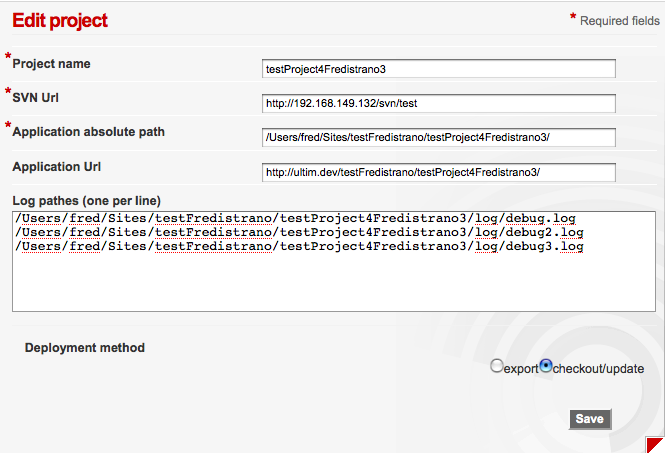
\includegraphics[width=1\textwidth]{doc_fredistrano1.png} 
\begin{enumerate}
\item Cliquer sur l'onglet "Projets" puis sur le lien "Ajouter un projet"
\item Renseigner les différents champs du formulaire de création :\\
\begin{list}{- Champ}{}
\item \textbf{"Nom du projet"} : Permet d'identifier le projet, servira également de nom pour un dossier temporaire lors du déploiement, il est donc préférable d'éviter les caractères spéciaux.
\item \textbf{"Url SVN"} :  Url vers le repository SVN du projet à déployer (exemple : "http://svn.mondomain.com/monProjet/trunk").
\item \textbf{"Chemin absolu du projet à déployer"} :  Chemin absolu vers le dossier sur le serveur de production où sera déployé l'application\\exemple sur un serveur Windows : D:\textbackslash www\textbackslash html\textbackslash monProjet \\exemple sur un serveur Linux : /var/www/html/monProjet ou encore /home/monUser/monDomain.com.
\item \textbf{"Url de l'application à déployer"} :  Servira uniquement à afficher un lien vers l'application.
\item \textbf{"Chemin des fichiers de log"} : Chemins des fichiers de log que vous souhaitez rendre accessible depuis le visualisateur de log, un chemin par ligne.
\item \textbf{"Méthode de déploiement"} : \textbf{Checkout/update:} méthode la plus rapide, lors du premier déploiement un "svn checkout" est exécuté pour les déploiements suivants la commande "svn update" sera utilisée qui récuperera uniquement les fichiers modifiés. \textbf{Export:} plus lent, car pour chaque déploiement la commande "svn export" est utilisée, cependant il est parfois nécessaire d'utiliser cette méthode, par exemple si vous n'avez pas les droits nécessaire sur le repository subversion pour exécuter la commande checkout.
\end{list}
\end{enumerate}




\subsection{Déploiement d'un projet}
\begin{enumerate}
\item Afficher le détail du projet à deployer
\item Cliquer sur "Déployer le projet".
\item Préciser le numéro de révision à déployer si nécessaire, pour la version la plus récente ne rien mettre.
\item Dans le cas d'un projet Subversion privé, protégé par mot de passe, préciser le login et mot de passe (si l'authentification est commune à tous vos projets à déployer, il est possible de renseigner le login et mot de passe subversion dans le fichier app/config/config.php ).
\item Cliquer sur "Step 1 SVN export"
\item La commande svn export est exécutée dans le dossier "Fredistrano/files/tmp/nomduprojet/tempDir".
\item Simulation coché rien ne sera fait, juste un résumé de ce qui va être fait sera affiché.
\item Cliquer sur "Step 2 synchronisation"
\item Un backup du répertoire de production est effectué dans "Fredistrano/files/backup/nomduprojet" puis la commande rsync est exécutée entre le dossier "Fredistrano/files/tmp/nomduprojet/tempDir" et le dossier "nomduprojet"
\item "Step 3 finalisation" les trois options sont désactivables: renommage des fichiers '.prd.', l'ajustement des droits des répertoires et fichiers et enfin les droits d'écriture sur les dossiers définis dans deploy.php.
\end{enumerate}

\subsection{Déploiement d'un projet en mode rapide}
\begin{enumerate}
\item Afficher le détail du projet à deployer.
\item Cliquez sur le lien "changement de mode de déploiement" pour changer le mode de déploiement, le bouton change de label : "Déploiement rapide".
\item Toutes les différentes étapes de déploiement seront exécutées automatiquement avec les options standards (renomage des fichiers prd, modification des droits uniquement sur les fichiers modifiés, droit d'écriture comme défini dans le fichier deploy.php). 
\end{enumerate}

\section{Logs de déploiement}
Vous pouvez accéder à l'historique de déploiement depuis la page détail de chaque projet en cliquant sur le lien "changement de mode de déploiement". Un flux rss est disponible dans le menu de droite sur cette page. Il est possible de désactiver les flux rss dans le fichier /app/config/config.php.

\section{Visualisateur de logs}
Cliquez sur l'onglet "Logs" pour accéder au visualisateur de log, grâce à cette fonctionnalité vous pourrez afficher le contenu des fichiers de log défini dans le détail des projets.

\section{Trucs et astuces}
\subsection{Commun à tous type de projet} % (fold)
\begin{list}{-}{}
\item \textbf{Exemple de script beforeScript}\\
Ce script permet de remplacer le .htaccess d'un projet par un autre .htaccess pendant l'étape de syncronisation d'un déploiement qui redirigera les visiteurs vers une page temporaire. Le fichier .htaccess temporaire et la page qui servira pour la redirection sont placés dans le dossier .fredistrano à la racine du projet

	\definecolor{lbcolor}{rgb}{0.9,0.9,0.9}
	\lstset{language=bash}
	\lstset{breaklines=true}
	\lstset{tabsize=1}
	\lstset{backgroundcolor=\color{lbcolor},rulecolor=}
	\begin{lstlisting}[frame=tb]{}
	#!/bin/sh

	PATHTMP=/Path/on/production/server/fredistrano/files/tmp/myproject/tmpDir
	PATHPRD=/Path/on/production/server/myproject

	# copy the specific temporary .htaccess at the right place 
	cp -vf ${PATHTMP}/.fredistrano/.htaccess ${PATHPRD}/.htaccess
	#  copy the specific temporary redirect page at the right place 
	cp -vf ${PATHTMP}/.fredistrano/302.html ${PATHPRD}/302.html
	\end{lstlisting}

\item \textbf{Exemple de script afterScript}\\
Ce script va changer une valeur dans un fichier, dans cet exemple il va mettre la configuration du mode debug à 0 dans le fichier app/config/core.php. Il va également remettre le fichier .htaccess que l'on a remplacé par un fichier temporaire pendant le déploiement et supprimer le fichier de redirection (voir l'exemple de script beforeScript) 
	\definecolor{lbcolor}{rgb}{0.9,0.9,0.9}
	\lstset{language=bash}
	\lstset{breaklines=true}
	\lstset{tabsize=1}
	\lstset{backgroundcolor=\color{lbcolor},rulecolor=}
	\begin{lstlisting}[frame=tb]{}
	#!/bin/sh
	# modify the debug mode from 1 or 2 to 0 in file app/config/core.php
	PATHTMP=/Path/on/production/server/fredistrano/files/tmp/myproject/tmpDir
	PATHPRD=/Path/on/production/server/myproject

	sed -i.bak "s/\('debug',\)[ ]*[12]/\1 0/g" ${PATHPRD}/app/config/core.php

	# replace the temporary .htaccess 
	cp -vf ${PATHTMP}/.htaccess ${PATHPRD}/.htaccess

	# remove the temorary redirection page 
	rm -vf ${PATHPRD}/302.html
	# remove the old version of app/config/core.bak
	rm -vf ${PATHPRD}/app/config/core.php.bak
	\end{lstlisting}


\end{list}
% subsection commun_à_tous_type_de_projet (end)

\subsection{Spécifiques aux projets basés sur CakePHP} % (fold)
\begin{list}{-}{}
	\item \textbf{Suppression du cache:} Pour vider le cache automatiquement à chaque déploiement, il faut versionner les dossiers app/tmp/cache/models, app/tmp/cache/persistent et app/tmp/cache/views mais ignorer leur contenu. De cette façon, pendant l'étape de synchronisation du processus de déploiement ces dossiers seront vidés sur le serveur de production.\\
	Pour ignorer le contenu de ces dossiers dans subversion, j'utilise la commande suivante en me placent à la racine du projet :
	\definecolor{lbcolor}{rgb}{0.9,0.9,0.9}
	\lstset{language=bash}
	\lstset{breaklines=true}
	\lstset{tabsize=1}
	\lstset{backgroundcolor=\color{lbcolor},rulecolor=}
	\begin{lstlisting}[frame=tb]{}
	svn propset svn:ignore "*" app/tmp/cache/models/ app/tmp/cache/persistent/ app/tmp/cache/views/ app/tmp/logs/ app/tmp/sessions/ app/tmp/tests/
	\end{lstlisting}
\end{list}
% subsection spécifiques_aux_projets_basés_sur_cakephp (end)

\chapter{Références}
\begin{itemize}
\item Un hébergement qui permet l'utilisation de Fredistrano \\ http://www.fbollon.net/node/12 \\
\item Un billet sur l'utilisation de Subversion \\ http://www.fbollon.net/node/65 \\
\item Le forum d'aide de Fredistrano \\ http://groups.google.com/group/fredistrano-discuss
\end{itemize}

\end{document}